\chapter{Introduction}\label{chapter:introduction}
Modern computer systems are facing various threats of being attacked. Users are one of the most commonly exploited things around computers, especially with social engineering and fishing. Most systems currently rely on a standard combination of username and password. In 2009, Aloul et al.\ described the most common security concerns with passwords:\cite{aloul2009two}
``Users tend to use easy-to-guess passwords, use the same password in multiple accounts, write the passwords or store them on their machines, etc. Furthermore, hackers have the option of using many techniques to steal passwords such as shoulder surfing, snooping, sniffing, guessing, etc.''

Furthermore, many users tend to stay logged into services with their mobile devices, despite not having appropriate security measures for their devices. On most Android phones, full disk encryption is not enabled by default, which leads to another attack vector for identity theft.

Aloul et al.\ introduced a system of \glspl{otp} using mobile phones, which significantly improves security by introducing a second factor of authentication. However, for authentication situations on smartphones themselves the \gls{otp} mechanism is rendered pretty much useless, as the second factor is in fact on the same device.

\section{Vision}
The whole vision of this thesis is to provide a way to easily detect individual users by a short authentication sequence based on acceleration patterns. Even though this does not necessarily qualify as cryptographically secure authentication, behavioural patterns and keystroke recognition can be used as biometric authentication aids. For example, Bhargav-Spantzel et al.\cite{bhargav2006privacy}\ described a system to extract cryptographic biometric keys from biometric data and how this can be combined with additional other proofs of identity to provide strong authentication.

With acceleration pattern recognition, we will make a authentication mechanism with zero additional user interaction possible. This allows for higher frequency user re-authentication without disturbing and annoying the user. That means, instead of prompting the user with a login screen every 24 hours, we can measure his or her acceleration patterns every time sensitive information is accessed. Therefore, we can not only provide basic login authentication, but also provide a way for users to stay authenticated for longer sessions or even detect when someone else hijacks a valid session. Since the time between two authentication requests can almost be arbitrarily small, an attacker who gets control over the current session will get a new authentication request relatively quickly, thus minimizing the potential damage.
\section{Single user licenses}
Another application of this technique is to identify individual users, even if using the same device. This might not only be useful in terms of individualizing the software according to the current user, but also for tracking of software usage.

A common licensing model for software are per-user licenses, i.e.\ $n$ licenses for $n$ users of the software. However, this license model currently cannot be enforced, since the software is installed on a single physical device, which may be shared among users. This led to most software companies licensing their software per-installation instead of per-user.
As of 2016, many users tend to have multiple devices and also want to use their licenses on multiple devices. This resulted in a trend to bind software licenses to user accounts instead of devices. This trend is also prevailing in modern \gls{saas} models, which do not require installation of the software on end-user devices anymore.
A possible circumvention of these account bound licenses is account sharing. This imposes a real problem, not only for software licensors, but also for other access providers. For example a consumer research from Parks Associates\cite{accountsharing} reports, that ``6\% [of video streaming users] are exclusively using shared accounts to access subscription''. 

The methods described in this theses can give a powerful way to detect individual users sharing physical devices, as well as sharing individual accounts and thus reduce copyright infringements that could not even be detected beforehand.

\section{Multi-factor authentication}
\gls{mfa} is a technique to enhance security in access control situations. It combines multiple forms of authentication mechanisms, based on conceptually different approaches: Knowledge, e.g.\ passwords or PINs; possessions, e.g.\ keys or bank cards and biometric characteristics, like fingerprints or, as in our approach, behavioural patterns.

A typical authentication attempt with \gls{mfa} is only successful, when all needed factors are present. The most common example for \gls{mfa} is banking, where one needs to be in possession of the banking card and needs to know the card's PIN. However, an attack vector targeting this system is copying the banking card while the attacked person does not notice his card being copied. This attack vector is also possible with biometric characteristics and even relatively easy, as many biometric traits are publicly visible. Fingerprints have proven to be copyable with low cost\cite{starbug2008bastel} and new high resolution cameras allow to photograph fingerprints and eyes in high enough quality to spoof many scanners\cite{fiebig2014security}. These attacks also can be adapted to other authentication systems based on visible biometric traits, such as iris recognition or Android's Face Unlock.

For biometric authentication to be sufficiently secure, the traits need to be intrinsic, i.e.\ not publicly visible, and hard to copy. Acceleration based motion detection matches these requirements, as recording of these patterns is only possible with physical access to the authentication device or very close monitoring of all body movement of the user.

\section{Smart mobile devices}
Smart devices are electronic devices, that feature wireless communication, e.g.\ WiFi or Bluetooth. Smart \emph{mobile} devices are smart devices, that are typically worn or kept in close proximity to the user. This usage usually results in small form factors and little weight. These devices are most often commodity devices and used frequently. Therefore, smart mobile devices are ideal to provide authentication, since the authenticating user is accustomed using the device.

\begin{figure}
    \centering
    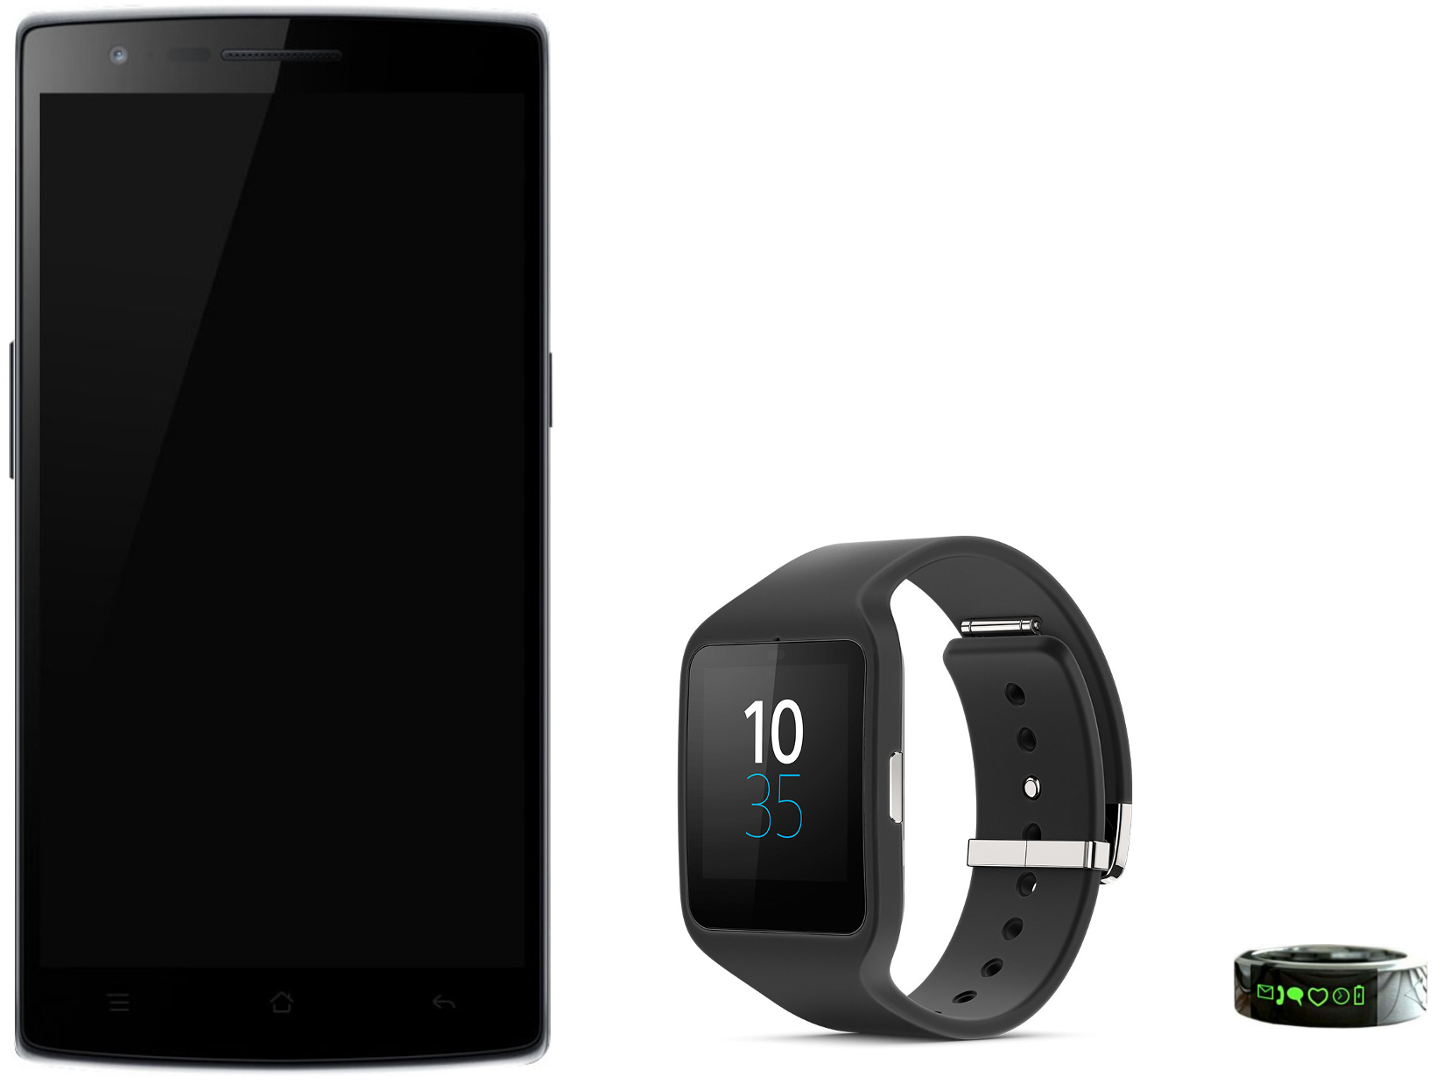
\includegraphics[width=0.8\textwidth]{figures/SmartDevices.png}
    \caption{Examples for smart mobile devices that are worn in close proximity of the user (from left to right): A OnePlus One smartphone, a Sony SmartWatch 3, Smarty Ring concept design}
    \label{fig:smartdevices}
\end{figure}
Currently common examples for smart mobile devices are smartphones. With the release of the Apple Watch last year in 2015, smartwatches increasingly became popular. With the increasing miniaturization of smart mobile devices, a consequent next step would be even smaller devices, like smart-rings. In Figure~\ref{fig:smartdevices} a size comparison between the three mentioned categories is shown.

\subsection{Smartphones}
Smartphones are the most capable of the smart mobile devices discussed herein. Smartphones usually have numerous wireless communication possibilities and thus function are a personal data-hub, to which other personal devices connect and communicate over. Typical connections for Smartphones are: Cellular network (e.g.\ \acrshort{gsm}, \acrshort{umts}), WiFi, Bluetooth, Near Field Communication etc. Smartphones are also packed with sensors, which can be utilized by programmers of \Glspl{app} and typically include acceleration as well as gyroscopic sensors for movement detection.

The three major operating systems on smartphones are Android, iOS and Windows. As shown in Figure~\ref{fig:smartphoneosmarketshare}, Android has the biggest market share of over 80\% and an \gls{app} targeting both Android and iOS can target up to 98\% of the smartphone audience.

\begin{figure}
    \centering
    \includestandalone[width=0.8\textwidth]{figures/smartphoneosmarketshare}
    \caption{Market share of smartphone operating systems in Q3'15\cite{gartner2015smartosmarketshare}}
    \label{fig:smartphoneosmarketshare}
\end{figure}

\subsection{Smartwatches}
Smartwatches, as displayed in the middle of Figure~\ref{fig:smartdevices}, are a much newer iteration of wearable smart mobile devices. Early designs for smartwatches came up in the 1980's and first prototypes were released in the 1990's. However, modern smartwatches feature network connectivity and are usually paired via Bluetooth with smartphones.

\begin{figure}
    \centering
    \includestandalone[width=0.8\textwidth]{figures/wristwearosmarketshare}
    \caption{Market share of wristware operating systems in 2015\cite{idc2015wristmarketshare}}
    \label{fig:my_label}
\end{figure}

The currently biggest market share with over 50\% in smartwatches has Apple, with its Apple Watch, running watchOS. Android Wear, an adapted version of the Android operating system for smartwatches, has the second highest market share. All in all, the smartwatch market is more diverse than the smartphone market, with several independently developed operating systems like Pebble OS or Samsumng's Tizen. However, Android Wear has the advantage of having the same programming interfaces as Android. 

With developing \glspl{app} for Android in combination with small adaptions to Android Wear, developers can target a huge percentage of smartphones and also can develop smartwatch apps with virtually no overhead.

\subsection{Smart-rings}
Smart-rings are the next step towards even smaller wearables. The basic concept of these rings is to provide ``smart'' basic functionality a smartwatch can provide, without the need to wear a watch. For example displaying notifications or providing authentication for payment processes can also be done solely on a smart ring.

However, there are no real commercially available smart-ring products yet, but just design concepts and prototypes. Specially developed smart-rings with acceleration sensors should be able to identify users based on their motion patterns. Future work might provide basic functionality on smart-rings, but definitely needs adaption to the special purpose operating systems. 

\section{Pattern recognition}
TODO: hier schaubild einfügen
\cite{bishop2006pattern}
\subsection{Preprocessing}
Practical applications -> preprocessing -> transform the data, so the problem will be easier to solve

Generally, scaled to a fixed size (e.g. digits to recognize) to have similar shape and location

result: predictable and uniform input

preprocessing -> operating on the raw acceleration sensors
\subsection{Feature extraction}
we make a distinction preprocessing vs. feature extraction -> FE extracts the relevant data for our specific use-case.

makes it much easier for a subsequent pattern recognition algorithm to distinguish between the different classes

no need to compare the whole input data set, but only the ``features'' -> computationally faster and smaller to store for authentication (dimensionality reduction)

comparable data needs to undergo the same preprocessing and feature extracting steps
handle with care: information is discarded, accuracy can decrease

\subsection{Classification}
(Seite 21, Bishop)
Training / learning phase

supervised vs. unsupervised

Once trained, can be used to determine the identity / class of a new value (test set) with generalization

final goal for this paper: clustering of similar datasets and identify the previously learned users.
Enhancement?: automatically cluster input data and identify, how many users are using the system